% !TeX spellcheck = en_US
\addscenariosection{1}{Clash Scenario}{Dragon Valley}{\images/dragon.png}

\begin{multicols*}{2}

\textbf{Author:} LAAMAKALA

%\textit{A valley where ancient dragons protect secrets long forgotten. Fight for power, claim the land, or perish like those before you.}

\textit{A valley of secrets long forgotten. Its heart belongs to the beasts of old, while its fringes lure the bold and the desperate. Fight for power, claim the land, or perish like those before you.}

% \textit{The valley calls to those who seek adventure and riches beyond imagination. Its heart is guarded by Dragons older than time, its edges lined with settlements of those who dare to claim a foothold in this perilous land. But there is no safety here—only the promise of power for those who fight, and the certainty of death for those who falter.}

\subsection*{\MakeUppercase{Scenario Length}}
This Scenario plays out over 13 Rounds 
%(or a shorter version over 9 Rounds).

\subsection*{\MakeUppercase{Player Setup}}
\textbf{Player Count:} 2 -- 4

\textbf{Starting Resources:} 14 \svg{gold}, 4 \svg{building_materials}, 1 \svg{valuables}

\textbf{Starting Income:} 10 \svg{gold}, 0 \svg{building_materials}, 0 \svg{valuables}

\textbf{Starting Units:}
\begin{itemize}
  \item pack of \svgunit{bronze} of second highest recruitment cost
  %\item A Pack of \svgunit{bronze} Units of the player's choice
\end{itemize}

\textbf{Town Buildings:}
\begin{itemize}
  \item \svgunit{bronze} Dwelling
  \item Each player may build the \svg{building_special_tent} building with a discount of 4 \svg{gold} and 2 \svg{building_materials}. % "Player Setup" -> discount is only before start of game.
\end{itemize}

\subsection*{\MakeUppercase{Map Setup}}
Take the following Map Tiles and arrange them as shown in the Scenario map layout ($P$ stands for the number of players):

\begin{itemize}
  \item P × Starting (I) Map Tile
  \item 3P × Far (II-III) Map Tiles - one per player must include a Settlement, and one per player must include a Trading Post
  \item 2P × Near (IV-V) Map Tile
  \item P × Center (VI-VII) Map Tiles (C5 is treated as a Settlement)
\end{itemize}

\textbf{Additionally, for 2--3 players:}
\begin{itemize}
  \item 1 × Center (VI-VII) Map Tile with a Dragon Utopia
\end{itemize}

\textbf{For 4 players:}
\begin{itemize}
  \item 2 × Center (VI-VII) Map Tiles with a Dragon Utopia
\end{itemize}

\subsection*{\MakeUppercase{Victory Conditions}}
The game ends at the end of the Round when any of these conditions are met:

\begin{itemize}
 \item One player has defeated each other player's Main Heroes once - \textit{That player wins the game immediately.}
 \item One player has conquered both Dragon Utopias %- \textit{That player wins the game immediately.}
 \item At the end of Round 13 (or Round 9 for the shorter game).
\end{itemize}

\subsection*{\MakeUppercase{Victory Points}}
If no player has achieved an immediate victory, the player with the most Victory Points (VP) wins:

\begin{itemize}
 \item 5 VP for conquering a Dragon Utopia
 \item 4 VP for controlling 5 Mines or Settlements on Near and Center Tiles - \textit{once per game}
 \item 4 VP for defeating an enemy's Main Hero - \textit{once per defeated Faction}
 \item 2 VP for defeating an enemy's Secondary Hero - \textit{once per defeated Faction}
 \item 2 VP for each enemy Main Town captured - \textit{once per captured Faction}
 \item 1 VP for every controlled Mine or Settlement
 \item 1 VP for every 2 Artifacts acquired during the game.
% \item 1 VP for every Level of Experience of your Main Hero
\end{itemize}

\subsection*{\MakeUppercase{Timed Events}}

\begin{itemize}
  \item[\textbf{\nth{1}}] \textbf{Round:} All Heroes gain +1 \svgeven{movement}.
  \item[\textbf{\nth{4}}] \textbf{Round:} Remove Black Cubes from all locations that give Resources, Morale or Cards (but not from the Grail).
  \item[\textbf{\nth{8}}] \textbf{Round:} Repeat event of Round 4.
  \item[\textbf{\nth{9}}] \textbf{Round:} Repeat event of Round 1.
  \item[\textbf{End}] \textbf{of \nth{10} Round:} Player(s) with lowest XP roll 2 \svg{resource} dice.
\end{itemize}

\subsection*{\MakeUppercase{Additional Rules}}
\begin{itemize}
  \item Remove ``View Earth'' from the Spell Deck.
  \item Remove ``Unexpected Reinforcements'' from the Astrologers Proclaim Deck.
  \item Create separate Decks for Minor, Major, and Relic Artifacts.
  \item Create separate Decks for Basic and Expert Spells.
  \item On Starting and Far Map Tiles, players can only acquire Basic Spells and Minor Artifacts. % To-do where to acquire expert spells?
  \item Sanctuary effect: \textbf{once per Faction} gain a \svg{morale_positive} token and draw 1 Card.
  \item Obelisk effect: \textbf{once per Faction} roll one \svg{resource} and draw one Card.
  
  \MakeUppercase{Battlefield Conditions} At the star of each Round, roll 2 Attack Dice: % Perhaps after the additional rules?
  \begin{itemize}
    \item "-1/-1": Dense Fog -- All Ranged units gain disadvantage. %\svg{unit_ranged} "gain" or "have?" "--" or ":"
    \item "-1/0": Torrential Rain -- All Flying Units gain -2 initiative. % \svg{unit_flying} \svg{initiative} from rulebook rewrite. / Or -1 movement on "Medium Hex Combat Board"
    \item "0/-1": Sinking Mud -- All Ground units have -1 Movement. %gain or have?
    \item "-1/+1": Scorching Earth -- All \svg{silver} and \svg{golden} Units start with 1 \svg{damage_red}
    \item "0/0": Clear Skies -- No effect. % or "calm before storm", "Sun is shining and birds are singing - " 
    \item "+1/-1": Fey Trickery -- Players Activate their Units in ascending order of Unit Initiative. %\svg{initiative}
    \item "0/+1": Rocky Terrain -- All Ground Units gain Shield Token. %\svg{defense}
    \item "+1/0": Tail Wind -- Flying Units gain +1 Movement. %\svg{unit_flying}
    \item "+1/+1": Perfect Conditions -- All Ranged Units gain advantage. %Or "Clear Skies" \svg{unit_ranged}
  \end{itemize} % Should this be made as a table?
  \textit{The same condition may not occur two rounds in a row.
  
  \item When fighting a Neutral Combat, a Player may add +1 difficulty only for an extra 5 \svg{gold} + Search (2) the Artifact or the Spell Deck. % could be moved to a timed event; Round 5: All Neutral Combats are considered +(I) on Far and Near Map tiles "
  \item Level VII Neutral fights cannot be skipped.
  \item If your Hero is Level VII, treat Level VI neutrals as Level VII, then gain 10 \svg{gold} for winning a Level VII Combat. % "and gain" / "and then gain" May be removed.
  \item Settlements on Center (VI-VII) Map Tiles count as two Settlements in terms of rewards AND allow rolling one \svg{resource} or \svg{treasure} (reroll any \svg{experience}).
  \item If a player's Main Hero defeats another Main Hero, the defeated Player may change a Defense Statistic Card to an Empowered Defense Card. % or - Defeated Main Hero may Empower one Defense Statistic Card ("from his Deck of M&M")
  \item Upon flagging a Grail Field, \textbf{choose one} and then put a Black Cube:
  \begin{itemize}
    \item Receive: 10 \svg{gold}, 4 \svg{building_materials}, and 2 \svg{valuables}.
    \item Roll 2 \svg{treasure} (reroll any \svg{experience}) and 2 \svg{resource}.
  \end{itemize}
  \item When visiting a Dragon Utopia: Reshuffle the \svgunit{golden} and \svgunit{azure} Decks, then draw from \svgunit{azure} until you get 3 Dragons and choose 2 (3 on impossible difficulty), AND draw from \svgunit{golden} until you get one Dragon.
  \item Upon flagging Dragon Utopia, \textbf{choose one} and then put a Faction Cube:
  \begin{itemize}
    \item Recruit one of the defeated Dragons for half its \svg{gold} (rounded down) and its \svg{valuables} cost.
    \item Receive 15 \svg{gold} AND Search (3) any Artifact Deck.
  \end{itemize}
  \item A Dragon Utopia can only be flagged once. A flagged Dragon Utopia is considered to be an empty field to all Players. % or: "Once flagged, it is treated as an empty field to all players."
\end{itemize}

After visiting a Dragon Utopia, roll an Attack Die:
\begin{itemize}
  \item[\textbf{-1}] -- Dragons' Curse: The defeated Dragons’ spirits curse the land! All Heroes lose \mbox{1 \svgeven{movement}} for the next Round.
  \item[\textbf{0}] -- Dragons' Revenge: All players must sacrifice a Unit before the end of the Round; that Unit's health is reduced to 0. 
  \item[ \textbf{+1}] -- Scattered Treasure: All players may immediately spend \mbox{1 \svgeven{movement}} to Search (2) the Artifact Deck.
\end{itemize}

\subsection*{\MakeUppercase{Suggested Houserules}}
\begin{itemize}
  \item Trading Posts - on a single visit, trade Resources and remove Cards, OR buy a War Machine.
%  \item Fighting Neutral Units entails the following:
%  \begin{itemize}
%    \item No Combat Round limit
%    \item On Hard+ difficulty, increase the difficulty of I-IV encounters by one
%    \item Gain Field Level × \svg{gold} as an additional reward
%  \end{itemize}
  \item \href{https://boardgamegeek.com/thread/3445901/custom-hex-combat-board}{Medium Hex combat board}.
  \item \href{https://boardgamegeek.com/thread/3449937/houserule-for-stacking-more-than-pack}{Stacking more than Pack} - Start with Several \svgunit{bronze} Units instead of Few.
\end{itemize}

\vspace*{\fill}

\end{multicols*}

\begin{tikzpicture}[overlay]
  \centering
  % 2-player
  \node at (4, -4) {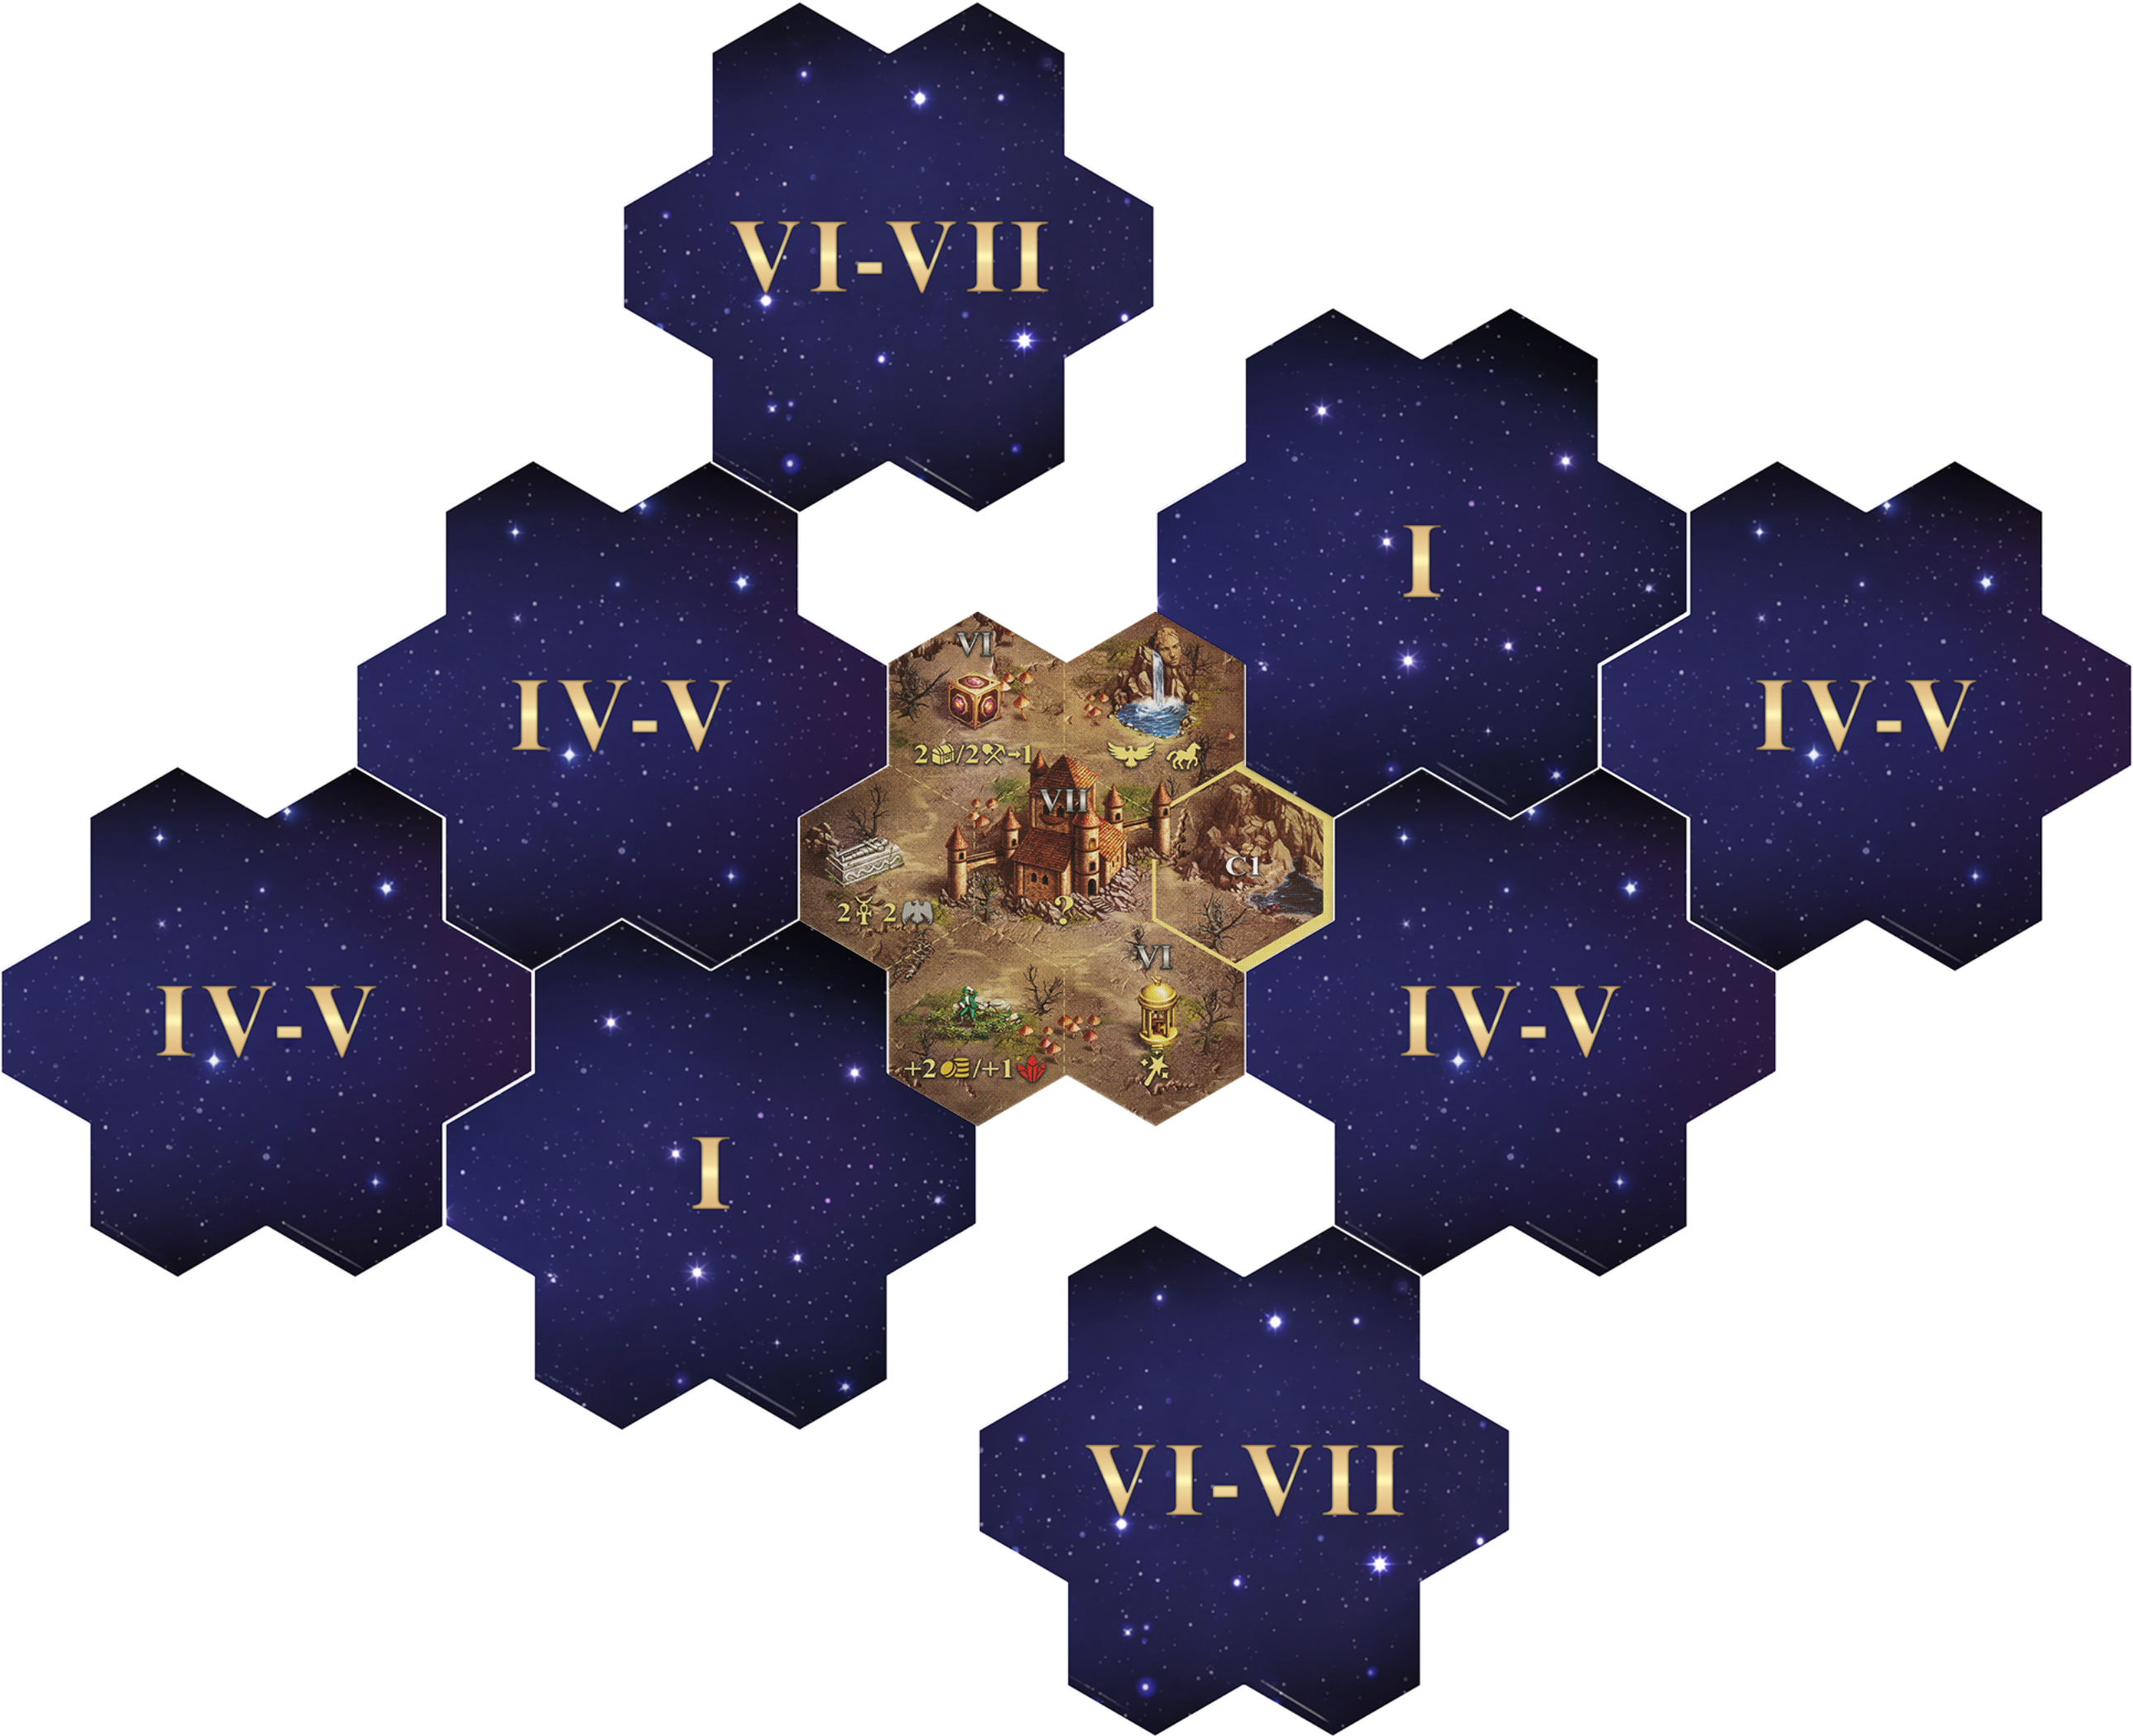
\includegraphics[scale=0.165]{\maps/dragon-valley-2p.png}};
  \node at (4, -9) {\footnotesize{\textbf{\MakeUppercase{2-PLAYER SCENARIO}}}};
  % 3-player
  \node at (13, -4) {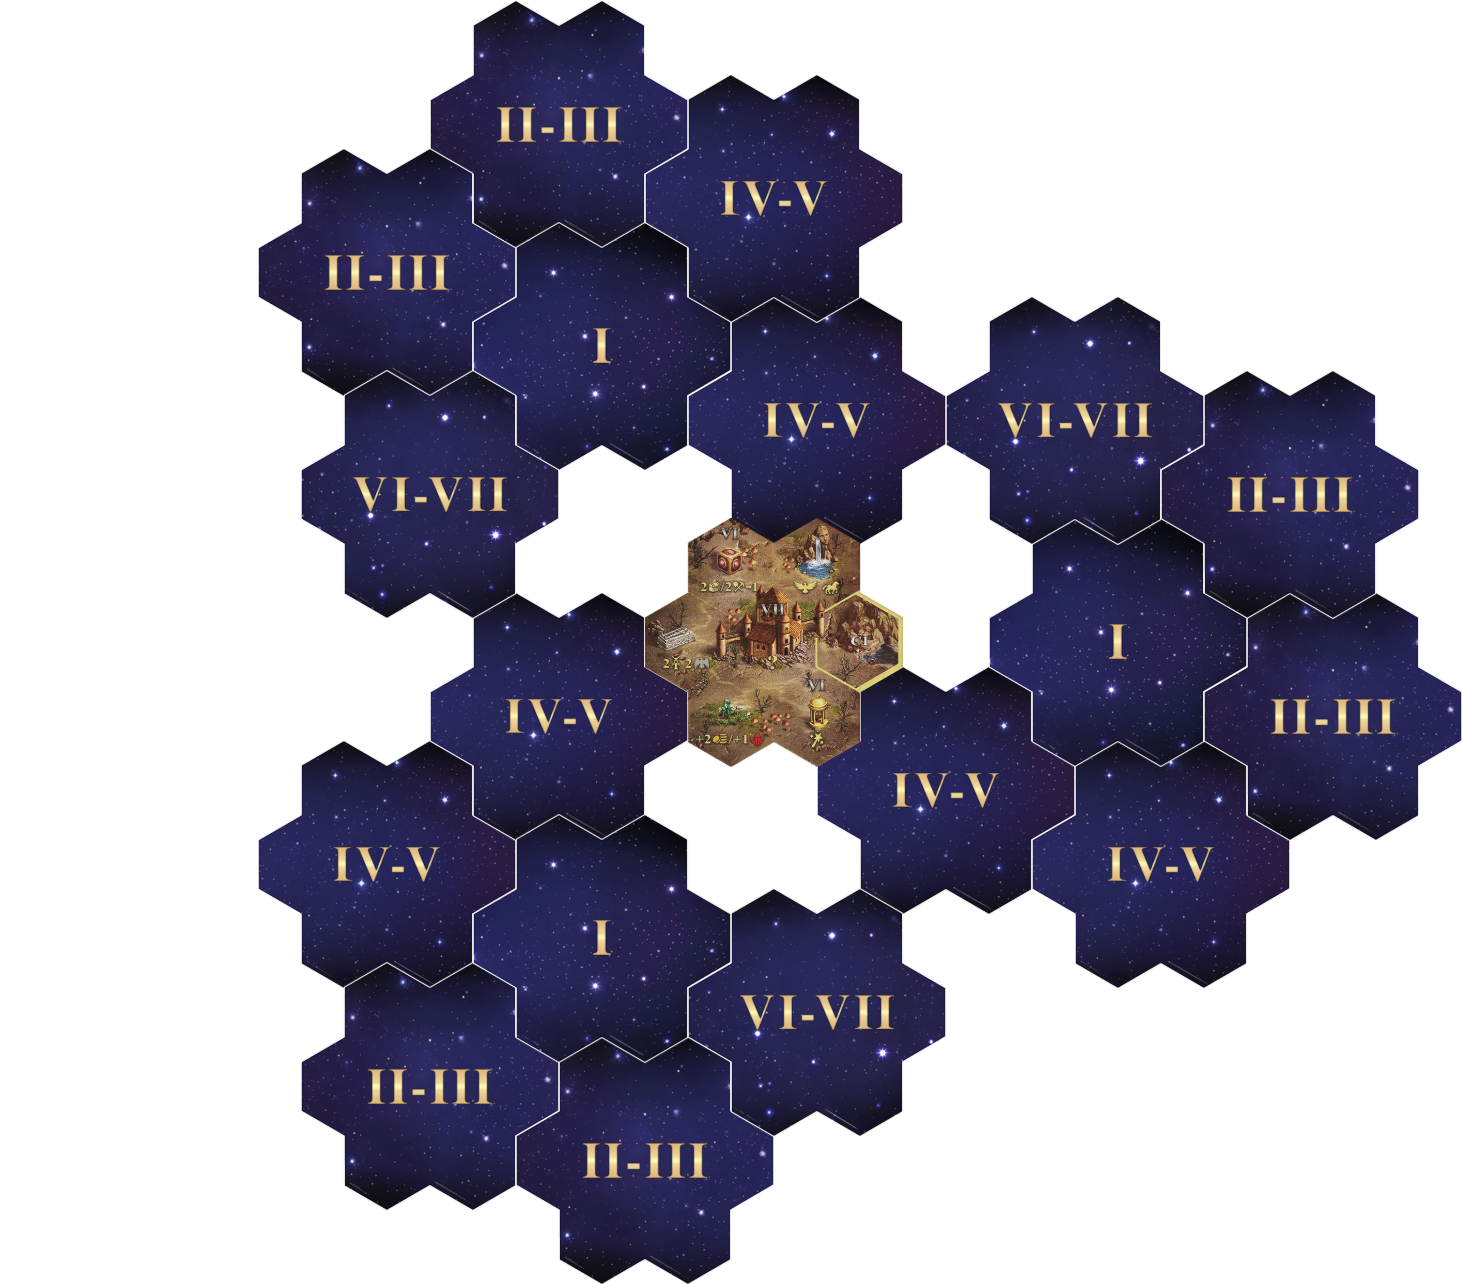
\includegraphics[scale=0.165]{\maps/dragon-valley-3p.png}};
  \node at (13, -9) {\footnotesize{\textbf{\MakeUppercase{3-PLAYER SCENARIO}}}};
  % 4-player
  \node at (4, -15) {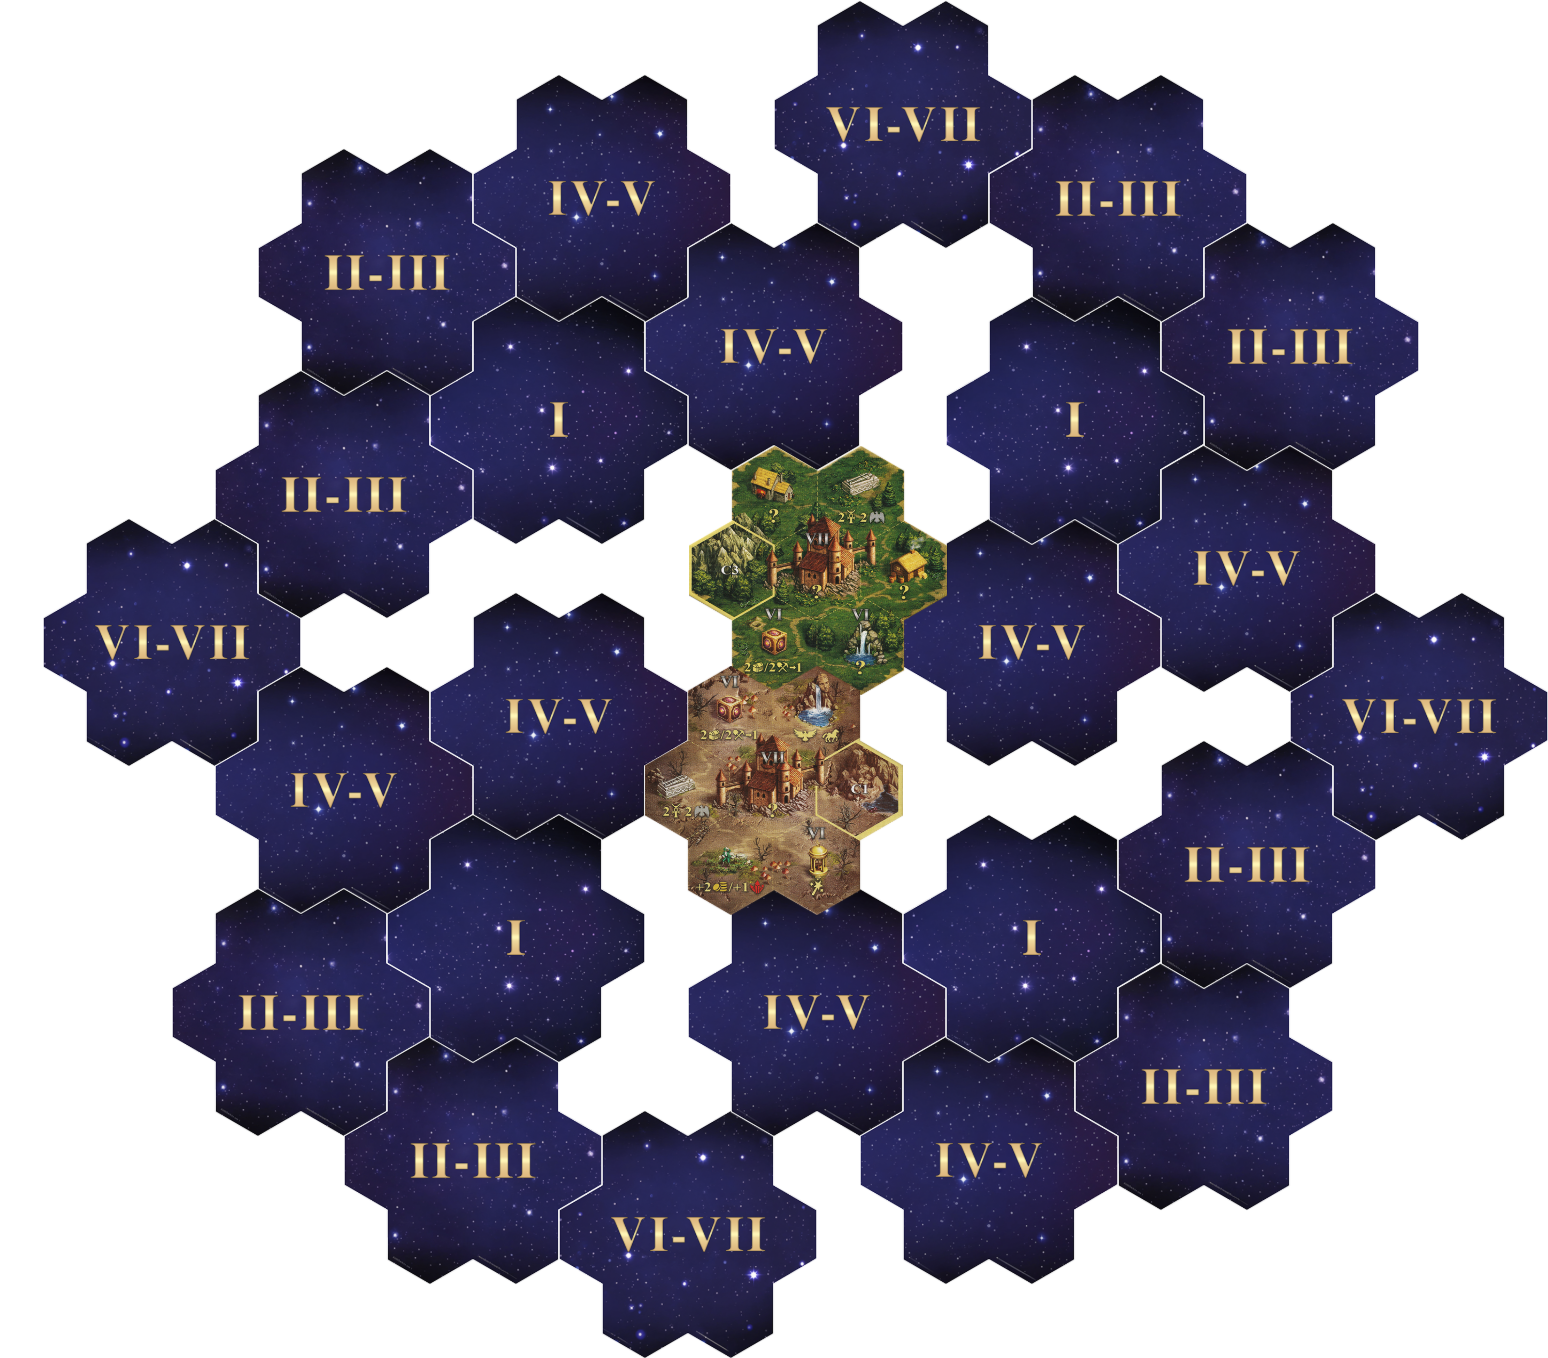
\includegraphics[scale=0.165]{\maps/dragon-valley-4p.png}};
  \node at (4, -20) {\footnotesize{\textbf{\MakeUppercase{4-PLAYER SCENARIO}}}};
  % 4-player short. -to be revised. Not tested.
  \node at (13, -15) {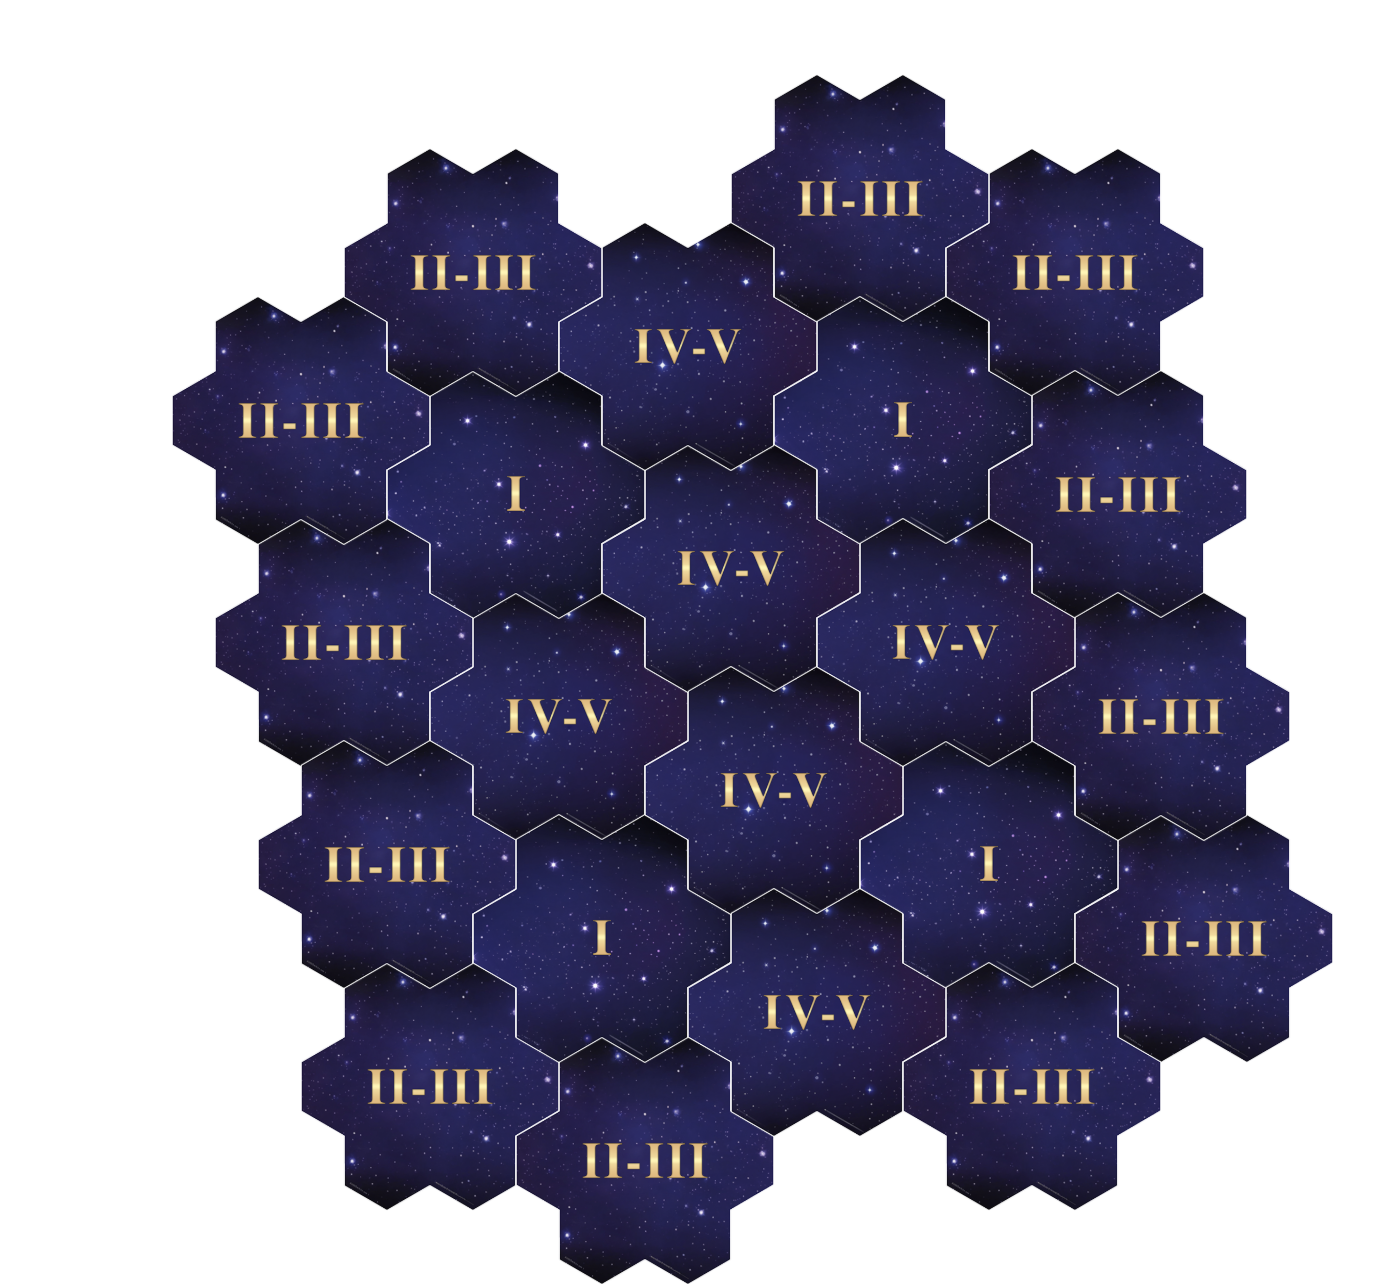
\includegraphics[scale=0.165]{\maps/dragon-valley-4p-short.png}};
  \node at (13, -20) {\footnotesize{\textbf{\MakeUppercase{4-PLAYER 9 ROUND SCENARIO}}}};
\end{tikzpicture}
